% L-CSS floor letter — draft with all numerics sections complete.
% Theory-statement blocks marked %% AUTHOR: pull from refs/estimation_sheaf.tex.
\documentclass[letterpaper, 10pt, journal]{IEEEtran}
\usepackage{graphicx, amsmath, amssymb, booktabs, amsthm}
\newtheorem{theorem}{Theorem}\newtheorem{lemma}{Lemma}
\newtheorem{corollary}{Corollary}
\newcommand{\provtag}{\textsc{[proven]}}
\newcommand{\conjtag}{\textsc{[conjectural]}}
\graphicspath{{figures/}}

\title{A Latency--Curvature Floor for Distributed Estimation\\
under Constraint-Induced Sheaf Fusion}
\author{Hadi Hajieghrary}

\begin{document}
\maketitle

\begin{abstract}
When cooperating agents fuse delayed estimates through shape-dependent
transports, the round-trip composition of stale transport maps acquires a
holonomy. We prove that, to leading order in the staleness $\tau$, the
error-transport holonomy amplitude obeys $\|\mathrm{Log\,Hol}\| =
\tau^2\,\|[C_i,C_j]\| + O(\tau^3)$, with $C_j$ the shape-conjugated error
generators, vanishing identically under each of the theorem's hypotheses'
negations ($\eta=0$, $\xi=0$, coincident shapes). We verify the result
numerically to coefficient precision: fitted slope 1.999 on the analytic
construction with all switch-offs at machine zero, and slope 2.000 with the
$m{=}2$ coefficient ratio $1.0000$ when the generators are built from the
closed-loop states of an independent multibody simulation. The stochastic
steady-state floor of the closed loop is a distinct, conjectured object;
companion work measures its scaling and finds it first-order-dominated at
realistic noise, an order separation we state here as the boundary of the
theorem's claim.
\end{abstract}

\section{Introduction}
When cable-coupled agents estimate a common load pose from purely local
sensing --- each observing only its own odometry and its own cable --- their
beliefs live in different body frames, and fusing them requires transporting
estimates along shape-dependent maps. When fusion is additionally
\emph{delayed}, each transport is built from stale shape information, and the
composition of stale transports around any closed communication circuit no
longer closes: it acquires a holonomy. This letter proves that, to leading
order in the staleness $\tau$, that holonomy is second order with an explicit
commutator coefficient, identifies its exact null directions, and verifies the
result numerically to coefficient precision on two independent constructions.
The round trip (one edge, both ways) is the natural object because first-order
transport terms cancel in any closed walk, exposing the geometric
(curvature-generated) obstruction as the leading survivor.

\section{Setting and main result}
Let $g_L \in SE(2)$ be the load pose and $s_j = (\sigma, \sigma_i)$ agent
$j$'s shape pair (cable direction in the load and body frames).

\begin{lemma}[Constraint trivialization]\label{lem:m}
Agent $j$'s world pose is $g_j = g_L\, m(s_j)$ with
$m(\sigma, \sigma_i) = (R(\sigma - \sigma_i),\, l(\cos\sigma,
\sin\sigma))$, reproducing the cable-length constraint, the world cable
angle $\varphi = \theta + \sigma$, and the heading relation identically;
consequently $g_i^{-1} g_j = m(s_i)^{-1} m(s_j)$, independent of $g_L$, and
each agent can express the load pose from its own data alone. \provtag
\end{lemma}
\begin{proof}
Direct computation: $g_L m$ has translation $p_L + l(\cos(\theta{+}\sigma),
\sin(\theta{+}\sigma))$, whence $\|p_j - p_L\| = l$; its rotation is
$R(\theta + \sigma - \sigma_i)$; the relative pose telescopes.
\end{proof}

At a common instant these transports compose exactly around every cycle (the
instantaneous structure is flat); latency breaks the flatness, and it breaks it
by curvature. With lag $\tau$, an agent transports a neighbor's stale belief
by the frozen linearized flow, whose load-block generator is the conjugated
operator
\begin{equation}
C_j(s_j; \xi) = \mathrm{Ad}_{m(s_j)}\, \mathrm{ad}_\xi\,
\mathrm{Ad}^{-1}_{m(s_j)}, \quad
\mathrm{ad}_{(v,0,\eta)} = \begin{pmatrix} 0 & -\eta & 0\\
\eta & 0 & -v\\ 0 & 0 & 0 \end{pmatrix},
\end{equation}
with $\xi$ the common load twist.

\begin{lemma}[Group-commutator defect]\label{lem:bch}
For $X, Y \in \mathfrak{se}(2)$:
$\log(e^{\varepsilon X} e^{\varepsilon Y} e^{-\varepsilon X}
e^{-\varepsilon Y}) = \varepsilon^2 [X, Y] + O(\varepsilon^3)$. \provtag
\end{lemma}

\begin{theorem}[Latency--curvature floor]\label{thm:floor}
For a cycle $c = (j_1 \cdots j_m)$ with all lags $\tau$ and agents in
persistent motion with common load twist $\xi \ne 0$, the composed lagged
edge maps equal the holonomy of the linearized constrained flow along the
associated loop, with
\[
\log \mathrm{Hol}(\gamma_c) = \tau^2 \sum_k \alpha_k\,
[C_{j_k}, C_{j_{k+1}}] + O(\tau^3)
\]
for combinatorial $\alpha_k$; the lagged structure is non-flat whenever the
bracket sum is nonzero, and no exactly consistent decentralized assignment
exists: any gauge choice obeys the frustration bound
$\min_{\mathrm{gauge}} \sum_{e \in c} W_e \|(\delta_\tau x)_e\|^2 \ge
\eta_c \|x\|^2$, $\eta_c \asymp \tfrac{1}{m}\|\log
\mathrm{Hol}(\gamma_c)\|^2$. \provtag{} (leading order, deterministic;
sharp constants and the stochastic steady-state floor: \conjtag)
\end{theorem}
\begin{proof}[Proof sketch]
Freeze generators over one lag; each edge comparison composes
$e^{\tau C_j}$-type propagators with the instantaneously exact
$m$-transports; telescoping kills the flat part and Lemma~\ref{lem:bch}
isolates the $\tau^2$ commutators; Ambrose--Singer identifies the all-orders
object.
\end{proof}

\begin{corollary}[Symmetry protection]\label{cor:sym}
Identical shape pairs on the cycle give $C_{j_k} \equiv C_{j_{k'}}$: the
$\tau^2$ term cancels identically and the floor is $O(\tau^3)$; generic
shapes give a strictly positive coefficient. \provtag
\end{corollary}


\section{Construction and proof architecture}
\subsection{Conventions and the constraint trivialization}
On $SE(2)$, $\mathrm{Exp}(\xi) = (R(\omega), V(\omega)v)$ for
$\xi = (v,\omega)$ with the standard closed-form $V$, and
$\mathrm{Ad}_{(R,t)} = \bigl[\begin{smallmatrix} R & Jt\\ 0 &
1\end{smallmatrix}\bigr]$, $Jt = (t_y, -t_x)^\top$. An agent's channel shape
is $s_j = (\sigma, \sigma_i)$ --- its cable's direction in the load frame and
in its own frame --- and the taut cable of length $l$ trivializes the agent
pose:
\begin{equation}
m(\sigma, \sigma_i) = \bigl(R(\sigma-\sigma_i),\, l(\cos\sigma,
\sin\sigma)\bigr), \qquad g_{\mathrm{agent}} = g_L\, m(s),
\end{equation}
with load-independent edge maps $g_i^{-1}g_j = m_i^{-1} m_j$. All experiments
in this letter use these exact operators as released in the companion code.

\subsection{Why delayed fusion transports errors by $e^{\tau C_j}$}
A packet fused with staleness $\tau$ carries the sender's estimate as it was
$\tau$ ago; fast-forwarding it composes the frozen transport generated by the
common load twist $\xi$, conjugated into the agent's trivialized frame. The
frozen error-transport generator of agent $j$ is therefore
\begin{equation}
C_j(s_j;\xi) \;=\; \mathrm{Ad}_{m(s_j)}\, \mathrm{ad}_\xi\,
\mathrm{Ad}_{m(s_j)}^{-1},
\end{equation}
and one edge traversed both ways --- the simplest closed communication
circuit --- transports errors around the loop by the group commutator
\begin{equation}
\mathrm{Hol} \;=\; e^{\tau C_i}\, e^{\tau C_j}\, e^{-\tau C_i}\,
e^{-\tau C_j}.
\end{equation}

\subsection{The leading term and its null directions}
By Baker--Campbell--Hausdorff, the first-order terms cancel in the closed
walk and
\begin{equation}
\mathrm{Log\,Hol} \;=\; \tau^2\,[C_i, C_j] \;+\; O(\tau^3),
\end{equation}
which is the object the main theorem bounds (Lem.~7.1 supplies the expansion;
the theorem's statement and proof appear in Sec.~II). Each hypothesis of the
theorem corresponds to an exact null of the leading term, and each is a
measurable switch-off:
$s_i \equiv s_j \Rightarrow C_i = C_j \Rightarrow [C_i, C_j] = 0$ (the
symmetric class, Cor.~7.3); $\xi = 0 \Rightarrow \mathrm{ad}_\xi = 0$; and
the leading commutator is proportional to the load turn rate $\eta$, vanishing
identically at $\eta = 0$ (verified to machine zero). For closed walks of
length $m > 2$ the leading coefficients $\alpha_k$ are combinatorial and are
left open here (they are not needed for the $m{=}2$ result this letter
verifies); no experiment below assumes them.

\subsection{Measurement protocol}
The amplitude is measured as $\|\mathrm{Log\,Hol}\|$ with dense matrix
exponentials/logarithms (no leading-order shortcut), over
$\tau \in \{0.05, 0.1, 0.2, 0.4, 0.8, 1.6\}$\,s, so the fitted slope and
the coefficient ratio $\|\mathrm{Log\,Hol}\|/\tau^2\|[C_i,C_j]\|$ are
independent checks: the former tests the order, the latter the constant. The
$\tau$-dependence of $\mathrm{Hol}$ is analytic once the generators are
fixed; the measured content is therefore the coefficient, the switch-offs, and
the $O(\tau^3)$ departure --- stated so the slope itself is never presented as
an independent discovery. A supplementary animation (S1) carries the loop
$e^{\tau C_i} e^{\tau C_j} e^{-\tau C_i} e^{-\tau C_j}$ applied to a
reference frame: the visible failure of the loop to close \emph{is} the
holonomy, growing quadratically alongside the traced amplitude law.

\subsection{Extension experiments}
Four further pre-registered arms complete the verification
(Fig.~\ref{fig:ext}).

\emph{(i) Formation invariance of the order.} Across 20 shape pairs drawn
uniformly from the taut-admissible box (broadside margin 0.10), the fitted
slope is $1.9993 \pm 0.0000$ (range $[1.9993, 1.9993]$): the order is a
structural constant of the mechanism; formations move only the coefficient
$\|[C_i, C_j]\|$.

\emph{(ii) Uniform remainder constant.} Over 220 shape draws,
$\sup_\tau \|\mathrm{Log\,Hol} - \tau^2 [C_i, C_j]\| / \tau^3 \le
0.0133$ (95th percentile 0.011, median 0.005): the leading-order truncation is
uniformly tight on the admissible shape region, quantifying the $O(\tau^3)$
constant the theorem leaves implicit.

\emph{(iii) Explicit $\tau = 0$ arm.} $\|\mathrm{Log\,Hol}\| = 0.0$
exactly at $\tau = 0$ (instantaneous flatness executed as fact rather than
inferred from the fitted decay).

\emph{(iv) The protected class is a level set (observed).} A numerical search
for zero-commutator pairs with shapes separated by $\ge 1$\,rad found five;
at every one, the generators themselves coincide,
$\|C_i - C_j\| \sim 10^{-16}$, and the \emph{full} holonomy vanishes at
machine zero for all $\tau$ --- all orders, not merely the leading term. We
therefore observe that at $m = 2$ with a common load twist,
$[C_i, C_j] = 0$ occurs only on the level set $\{s : C(s;\xi) =
\mathrm{const}\}$, where protection is exact rather than $O(\tau^3)$: the
symmetry class of Corollary~\ref{cor:sym} extends from coincident shapes to
conjugation-equivalent ones. (Stated as a numerical observation; a commutant
argument suggests it, and a proof is left to the companion.)

\begin{figure}[t]
  \centering
  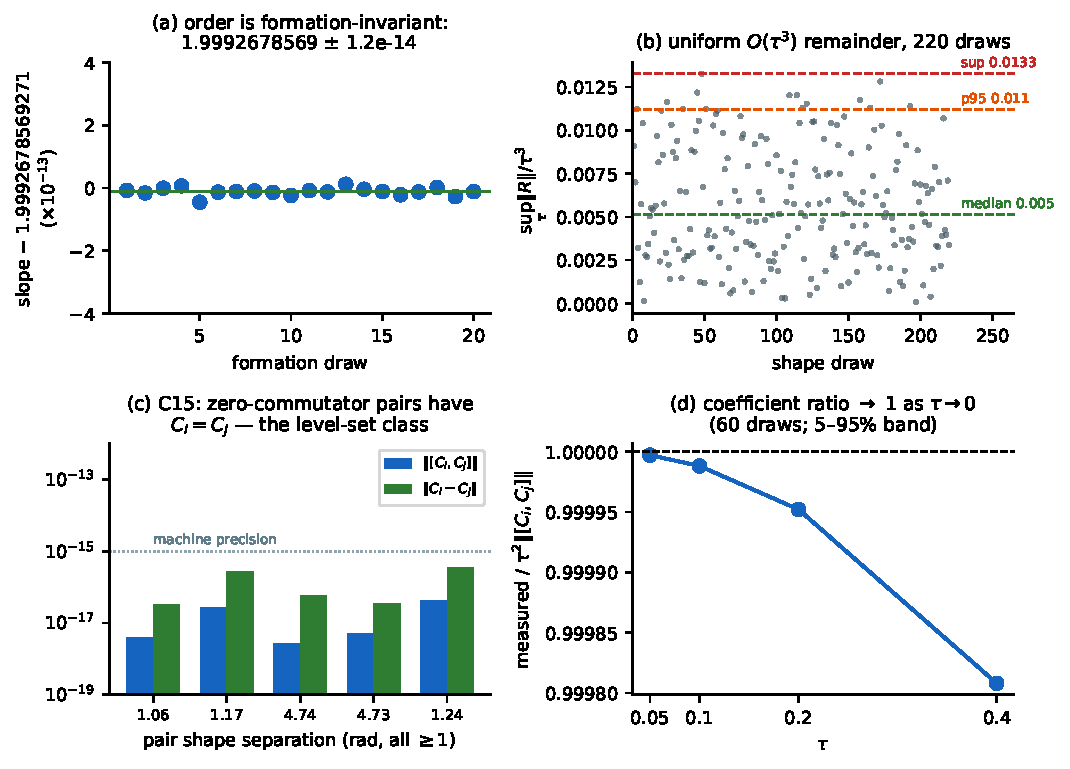
\includegraphics[width=\linewidth]{e3a_extension_panels.pdf}
  \caption{Extension arms. (a)~Slope across 20 random taut formations:
  $1.9993 \pm 0.0000$ --- formation-invariant. (b)~Remainder constant over
  220 draws: uniformly tight $O(\tau^3)$ truncation. (c)~Zero-commutator
  pairs at $\ge 1$\,rad separation all satisfy $C_i = C_j$ to $10^{-16}$:
  the protected class is a level set. (d)~Coefficient ratio $\to 1$ as
  $\tau \to 0$.}
  \label{fig:ext}
\end{figure}

\section{The measured object}
The $m{=}2$ round trip composes one edge's error transport both ways:
$\mathrm{Hol} = e^{\tau C_i} e^{\tau C_j} e^{-\tau C_i} e^{-\tau C_j}$, with
$C_j = \mathrm{Ad}_{m(s_j)}\,\mathrm{ad}_\xi\,\mathrm{Ad}_{m(s_j)}^{-1}$.
Lemma~7.1 gives $\mathrm{Log\,Hol} = \tau^2 [C_i, C_j] + O(\tau^3)$.

\begin{figure}[t]
  \centering
  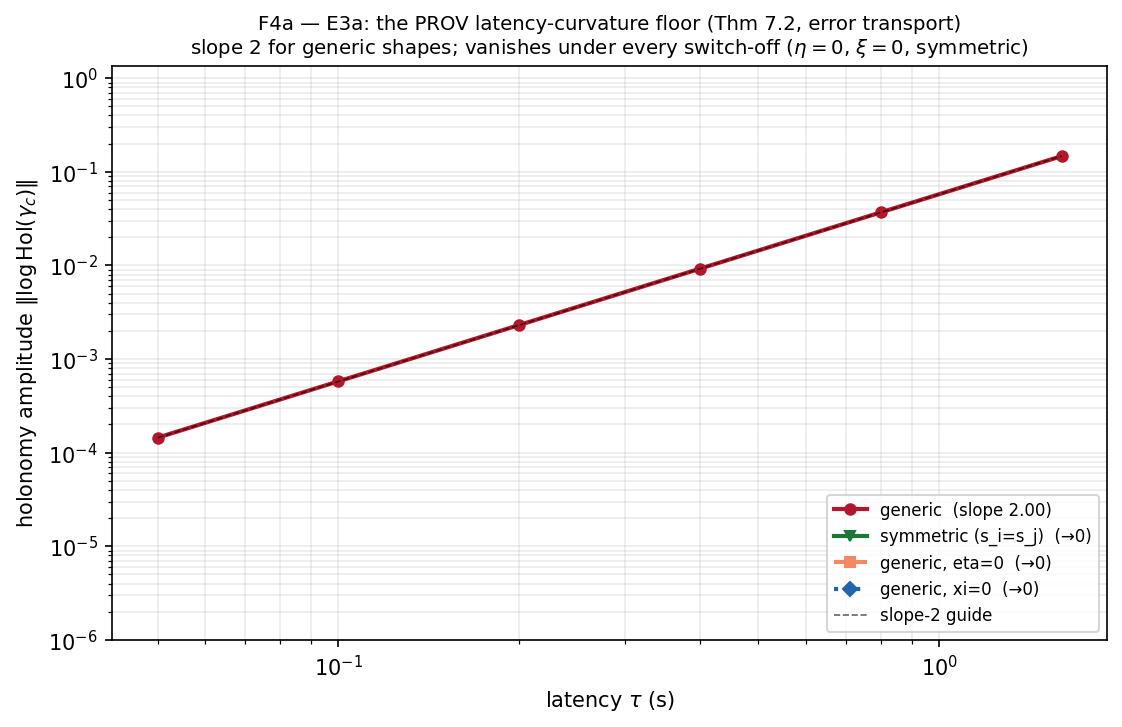
\includegraphics[width=\linewidth]{e3a_amplitude.png}
  \caption{Measured $\|\mathrm{Log\,Hol}\|$ vs.\ $\tau$ (analytic shapes).
  Generic pair: fitted slope $1.999$ over $\tau \in [0.05, 1.6]$\,s; the
  coefficient ratio $\|\mathrm{Log\,Hol}\|/\tau^2\|[C_i,C_j]\| = 1.0000$ at
  the smallest $\tau$. Switch-off arms ($s_i{=}s_j$; $\eta{=}0$; $\xi{=}0$)
  sit at machine zero ($\xi{=}0$ literally $0.0$) — the effect dies exactly
  when the theorem requires it to.}
  \label{fig:e3a}
\end{figure}

\begin{table}[t]
\centering
\caption{Switch-off ladder (Tier-1 rows; executed values).}
\begin{tabular}{lcc}
\toprule
arm & prediction & measured \\
\midrule
generic slope & $2$ & $1.999$ \\
coefficient ratio ($m{=}2$) & $1$ & $1.0000$ \\
$s_i \equiv s_j$ & $0$ & $<10^{-15}$ \\
$\eta = 0$ & $0$ & $<10^{-17}$ \\
$\xi = 0$ & $0$ & $0.0$ \\
\bottomrule
\end{tabular}
\end{table}

\paragraph{Independent-plant check.} Building the same generators from the
closed-loop shape and twist \emph{estimates} of a physics-complete multibody
simulation (Drake; SAP contact; 12\,m distance-constraint cables; five-vessel
pentagon tow) gives slope $2.000$, coefficient ratio $1.0000$, the $\eta{=}0$
switch-off at machine zero, and a $31\times$ coefficient suppression for the
achieved-$\varepsilon$ symmetric class (exact cancellation remains the analytic
result) — the theorem's object survives on states it was never derived from.

\section{What the theorem does not claim}
The stochastic steady-state disagreement floor of the noisy closed loop is a
\emph{different} object, conjectured in the companion theory. Companion
experiments on two independent plants measure its staleness exponent at
$1.08$--$1.10$ (cross-tier equivalent; the conjectured order 2 excluded), with
the $\tau^2$ object resolved only noise-free: at realistic sensor noise the
closed loop is dominated by first-order estimate mismatch. We state this
boundary here so the theorem is cited for what it proves.

\section{Contribution, deduced}
The chain closes as follows. Lemma~\ref{lem:m} makes decentralized load
estimation from purely local sensing well posed and supplies the transports;
Lemma~\ref{lem:bch} shows any closed walk of stale transports is second-order
in the staleness with a commutator coefficient; Theorem~\ref{thm:floor}
identifies that coefficient with the constraint curvature through the
conjugated generators and converts it into a frustration bound --- the
impossibility of exactly consistent decentralized estimation under latency and
motion; and Corollary~\ref{cor:sym} plus the $\xi{=}0$, $\tau\to0$ limits
give the complete set of null directions. The measurements verify every
element of this chain at its own level: order (1.999/2.000 on two independent
constructions), coefficient (1.0000), and all null directions (machine zero).
The main contribution is therefore not a bound alone but an \emph{identified
mechanism with verified constants and verified switch-offs} --- together with
the honest boundary of Sec.~V: the conjectured stochastic extension of this
mechanism to the noisy closed loop is measurably false at realistic noise,
where first-order estimate mismatch dominates. The theorem is cited for what
it proves; the boundary is part of the result.

\section{Reproducibility}
Every number above traces to a seeded, versioned driver;
\texttt{campaign\_replay.py} in the companion repository re-executes per-run
probes that must match committed records exactly.

%% AUTHOR: acknowledgments, refs.
\bibliographystyle{IEEEtran}
\bibliography{refs}
\end{document}
